%
% idee.tex -- Polynom Idee
%
\section{Idee
\label{reedsolomon:section:idee}}
\rhead{Problemstellung}
Um beim Datenübertragen Fehler zu erkennen, könnte man die Daten jeweils doppelt senden,
und so jeweilige Fehler zu erkennen.
Doch nur schon um Fehler zu erkennen werden überproportional viele Daten doppelt und dreifach gesendet.
Der Reed-Solomon-Code macht dies auf eine andere, clevere Weise.
Das Problem liegt darin Informationen, Zahlen, 
zu Übertragen und Fehler zu erkennen.
Speziell beim Reed-Solomon-Code kann man nicht nur Fehler erkennen, 
man kann sogar einige Fehler korrigieren.
Der Unterschied des Fehler erkennen und korrigiren, ist das beim Erkennen nur die Frage beantwortet wird: Ist die Übertragung fehlerhaft oder nicht?
Beim Korrigieren werden Fehler erkannt und dann zusätzlich noch den original Wert rekonstruieren.
Auch eine Variante wäre die Daten nach einer Fehlerhaften sendung, nochmals zum senden auffordern(auch hier wird doppelt und dreifach gesendung), 
was bei Reed-Solomon-Code-Anwendungen nicht immer sinnvoll ist. 
Anwendungen finden sind im Abschnitt \externaldocument{papers/reedsolomon/anwendungen}
\ref{reedsolomon:section:anwendung} beschrieben.

\subsection{Polynom-Ansatz
\label{reedsolomon:section:polynomansatz}}
\rhead{Polynom-Ansatz}
Eine Idee ist, aus den Daten ein Polynom zu bilden.
Diese Polynomfunktion bei bestimmten Werten errechnet und diese Punkte dann überträgt.
\begin{beispiel} Nehmen wir die Zahlen \textcolor{blue}{2}, \textcolor{blue}{1}, \textcolor{blue}{5},
welche uns dann das Polynom 
\begin{equation}
p(x)
=
\textcolor{blue}{2}x^2 + \textcolor{blue}{1}x + \textcolor{blue}{5}
\label{reedsolomon:equation1}
\end{equation}
ergeben.
Übertragen werden nun die \textcolor{darkgreen}{grünen Werte} 
dieses \textcolor{blue}{blauen Polynomes} an den Stellen 1, 2, 3\dots 7 dieses Polynomes.
Grafisch sieht man dies dann in Abbildung \ref{fig:polynom}, 
mit den Punkten, $p(1),p(2),...,p(7) = (\textcolor{darkgreen}{8}, 
\textcolor{darkgreen}{15}, \textcolor{darkgreen}{26},
\textcolor{darkgreen}{41}, \textcolor{darkgreen}{60}, 
\textcolor{darkgreen}{83}, \textcolor{darkgreen}{110})$
Wenn ein Fehler sich in die Übertragung eingeschlichen hat, muss der Leser/Empfänger diesen erkennen und das Polynom rekonstruieren.
Der Leser/Empfänger weiss, den Grad des Polynoms und dessen \textcolor{darkgreen}{Werte} übermittelt wurden. 
Die Farbe blau brauchen wir für die \textcolor{blue}{Daten} welche wir mit der Farbe grün \textcolor{darkgreen}{Übermitteln}.
\end{beispiel}

\begin{beispiel}
Ein Polynome zweiten Grades ist durch drei Punkte eindeutig bestimmbar.
Hat es Fehler in der Übertragunge gegeben,in der Abbilbung \ref{fig:polynom} die \textcolor{red}{roten Punkte}).
Erkennt man diese Fehler, da alle korrekten Punkte auf der Parabel liegen müssen. 
Die \textcolor{darkgreen}{grünen Punkte} bestimmen die Parabel, und die Fehler können zu den 
\textcolor{gray}{Orginalpunkte} rekonstruiert werden.
Ab wie vielen Fehler ist das Polynom nicht mehr erkennbar beim Übertragen von 7 Punkten?
Bei 2 Fehlern kann man noch eindeutig bestimmen, dass das Polynom mit 4 Punkten,
gegenüber dem mit 5 Punkten falsch liegt. \ref{fig:polynom}
Werden es mehr Fehler kann nur erkannt werden, dass das Polynom nicht stimmt.
Das orginale Polynom kann aber nicht mehr gefunden werden.
Da andere Polynome oder das Konkurrenzpolynom, grau gestrichelt in Abbildung \ref{fig:polynom}, das orginal fehlleitet.
Um das Konkurrenzpolynom auszuschliessen, währen mehr \textcolor{darkgreen}{Übertragungspunkte} nötig.
\end{beispiel}

\begin{figure}%[!ht]
	\centering
	%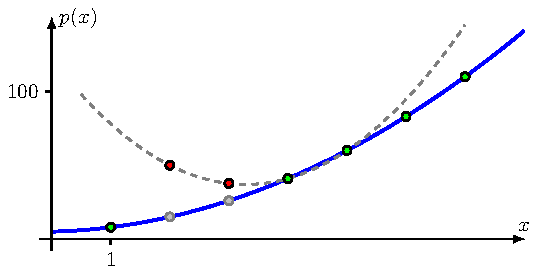
\includegraphics[width=\textwidth]{papers/reedsolomon/figures/polynom2}
    % polynomraw

\newcommand{\teiler}{40}


%//////////////////////////////////////

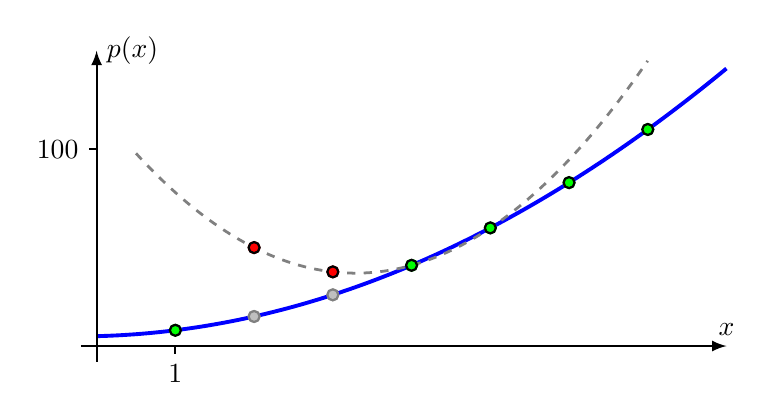
\begin{tikzpicture}[>=latex,thick,]
	\draw[color=blue, line width=1.4pt] 
	plot[domain=0:8, samples=100]
	({\x},{(2*\x^2+1*\x+5)/\teiler});

	\draw[->] (-0.2,0) -- (8,0) coordinate[label={$x$}];
	\draw[->] (0,-0.2) -- (0,150/\teiler) coordinate[label={right:$p(x)$}];
	
	\def\punkt#1{
		\fill[color=green] #1 circle[radius=0.08];
		\draw #1 circle[radius=0.07];
	}

	\def\hellpunkt#1{
		\fill[color=lightgray] #1 circle[radius=0.08];
		\draw[gray] #1 circle[ radius=0.07];
	}
	
	\draw[color=gray,line width=1pt,dashed] 
	plot[domain=0.5:7, samples=100]
	({\x},{(7.832*\x^2-51.5*\x+121.668)/\teiler});


	\punkt{(1,8/\teiler)}
	\hellpunkt{(2,15/\teiler)}
	\hellpunkt{(3,26/\teiler)}
	\punkt{(4,41/\teiler)}
	\punkt{(5,60/\teiler)}
	\punkt{(6,83/\teiler)}
	\punkt{(7,110/\teiler)}
	

	
	\def\erpunkt#1{
		\fill[color=red] #1 circle[radius=0.08];
		\draw #1 circle[radius=0.07];
	}
	\erpunkt{(2,50/\teiler)}
	\erpunkt{(3,37.66/\teiler)}

	\draw(0,100/\teiler) -- (-0.1,100/\teiler) coordinate[label={left:$100$}];
	\draw(1,0) -- (1,-0.1) coordinate[label={below:$1$}];		
\end{tikzpicture}
	\caption{Polynom $p(x)$ von der Gleichung\eqref{reedsolomon:equation1}}
	\label{fig:polynom}
\end{figure}

\section{Fehlerkorekturstellen bestimmen
\label{reedsolomon:section:Fehlerkorrekturstellen}}
Um zu bestimmen wieviel zusätzliche \textcolor{darkgreen}{Übertragungspunkte} notwendig sind, um die Fehler zu korrigieren,
muss man zuerst wissen, wieviel \textcolor{blue}{Daten} gesendet und wieviel \textcolor{red}{Fehler} erkennt werden sollen. 
Die Anzahl \textcolor{blue}{Daten} (ab hier verwenden wir das Wort Nutzlast), die als Polynomkoeffizente $k$ übergeben werden, 
brauchen die gleiche Anzahl an Polynomkoeffizententräger, beginnend bei Grad 0 somit ergibt sich der Polynomgrad mit $k-1$.
Für die Anzahl der Fehler $t$, welche korrigiert werden können, gehen wir zum Beispiel.
\begin{beispiel} von den Polynom \ref{reedsolomon:equation1} in, welchem wir  \textcolor{darkgreen}{7 Übertragungspunkte} senden.
Durch 3 Punkte wird das Polyom eindeutig bestimmt, nun haben wir mehrere Konkurrenzpolynome, doch mit maximal 2 Fehler liegen auf einem Konkurrenzpolynom,
maximal 4 Punkte und auf unserem orginal 5 Punkte. Ansonsten hatt es mehr Fehler oder unser Konkurrenzpolynom ist das gleiche wie das Original. 
Somit können wir nun bestimmen, dass von den \textcolor{darkgreen}{7 Übertragungspunkten$u$} bis zu 2 Fehler korrigiert werden können und 4 Übertragungspunkte zusätzlich gesendet werden müssen.
\end{beispiel}
Man könnte auch dies in der Tabelle \ref{tab:fehlerkorrekturstellen} erkennen, doch mit dieser Gleichung
\begin{equation}
    \frac{\textcolor{darkgreen}{u}-\textcolor{blue}{k}}{\textcolor{red}{t}}
    =2
    \label{reedsolomon:equation2}
\end{equation}
zeigt sich, dass es $k+2t$ Übertragungspunkte braucht.

\begin{table}
    \centering
    \begin{tabular}{ c c | c} 
        \hline
        Nutzlas & Fehler & Übertragen \\
        \hline 
        3 & 2 & 7 Werte eines Polynoms vom Grad 2 \\ 
        4 & 2 & 8 Werte eines Polynoms vom Grad 3 \\
        3 & 3 & 9 Werte eines Polynoms vom Grad 2 \\ 
        \hline
        $k$ & $t$ & $k+2t$ Werte eines Polynoms vom Grad $k-1$ \\ 
        \hline
    \end{tabular}
    \caption{ Fehlerkorrekturstellen Bestimmung.}
    \label{tab:fehlerkorrekturstellen}
\end{table}

Ein Nebeneffekt ist, dass dadurch auch $2t$ Fehler erkannt werden können, nicht aber korrigiert.
Um aus den übertragenen Zahlen wieder die Nutzlastzahlen zu bekommen könnte man eine Polynominterpolation anwenden,
doch die Punkte mit Polynominterpolation zu einem Polynom zu rekonstruieren ist schwierig und fehleranfällig.

